\documentclass[11pt]{book}
\usepackage{palatino}
\usepackage{amsfonts,amsmath,amssymb}
% \usepackage{graphicx}

\usepackage{listings}
\usepackage{textcomp}
\usepackage{color}

\definecolor{dkgreen}{rgb}{0,0.6,0}
\definecolor{gray}{rgb}{0.5,0.5,0.5}
\definecolor{mauve}{rgb}{0.58,0,0.82}

\lstset{frame=tb,
  language=R,
  aboveskip=3mm,
  belowskip=3mm,
  showstringspaces=false,
  columns=flexible,
  basicstyle={\small\ttfamily},
  numbers=none,
  numberstyle=\tiny\color{gray},
  keywordstyle=\color{blue},
  commentstyle=\color{dkgreen},
  stringstyle=\color{mauve},
  breaklines=true,
  breakatwhitespace=true,
  tabsize=3
}



\ifx\pdftexversion\undefined
    \usepackage[dvips]{graphicx}
\else
    \usepackage[pdftex]{graphicx}
    \usepackage{epstopdf}
    \epstopdfsetup{suffix=}
\fi

\usepackage{subfig}

\begin{document}

%%%%%%%%%%%%%%%%%%%%%%%%%%%%%%%%%%%%%%%%
% Problem Set 6
%%%%%%%%%%%%%%%%%%%%%%%%%%%%%%%%%%%%%%%%

\pagestyle{empty}
{\noindent\bf Spring 2021 \hfill Firstname M.~Lastname}
\vskip 16pt
\centerline{\bf University of Central Florida}
\centerline{\bf College of Business}
\vskip 16pt
\centerline{\bf QMB 6911}
\centerline{\bf Capstone Project in Business Analytics}
\vskip 10pt
\centerline{\bf Solutions:  Problem Set \#6}
\vskip 32pt
\noindent


%%%%%%%%%%%%%%%%%%%%%%%%%%%%%%%%%%%%%%%%
% Density Plots and Q-Q Plots
%%%%%%%%%%%%%%%%%%%%%%%%%%%%%%%%%%%%%%%%


\pagebreak
\section*{Probability Density Function of Fly Reel Prices}

Figure \ref{fig:density_prices} shows  the kernel-smoothed probability density function of fly reel prices.

\begin{figure}[h!]
  \centering
  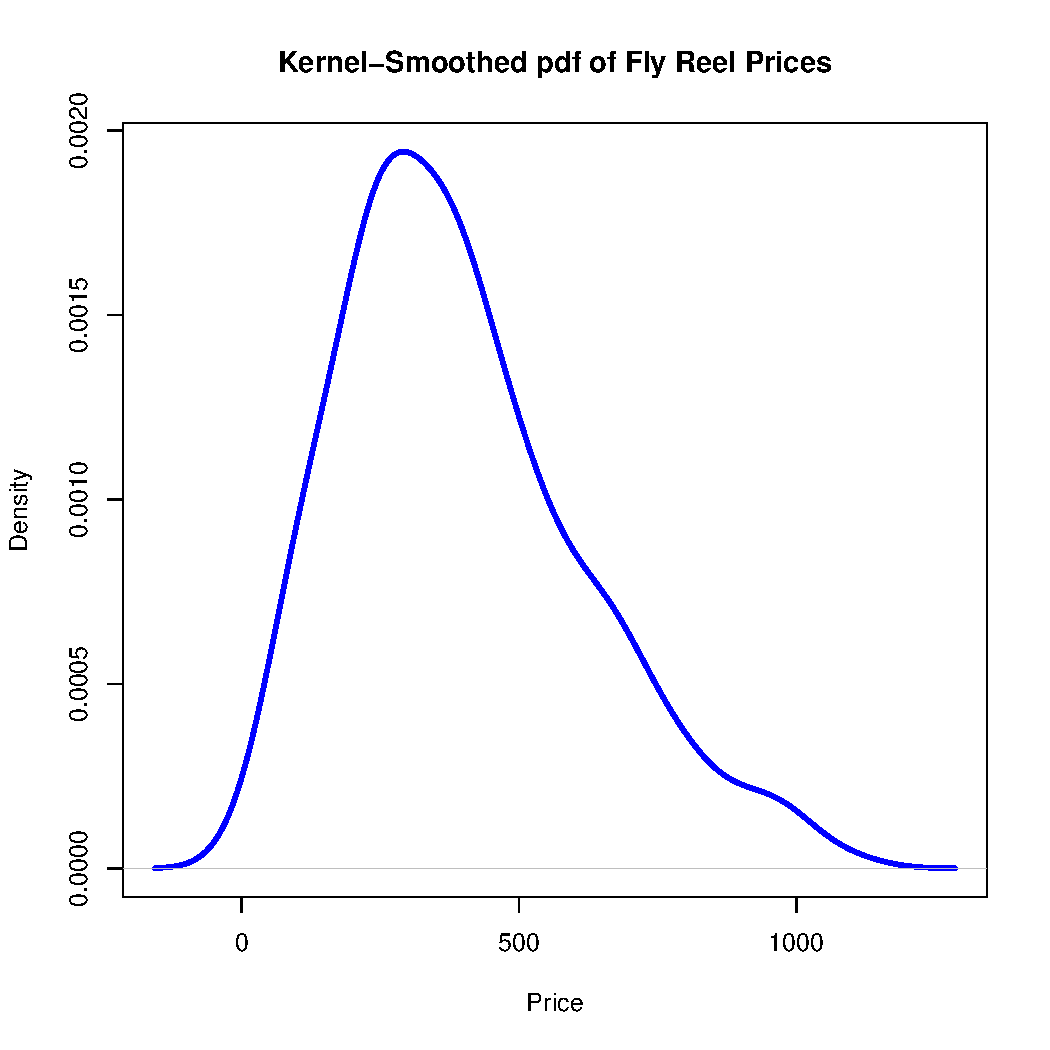
\includegraphics[scale = 0.5, keepaspectratio=true]{../Figures/density_prices}
  \caption{Probability Density Function of Fly Reel Prices} \label{fig:density_prices}
\end{figure}



\pagebreak
As a comparison, Figure \ref{fig:density_log_prices} shows the kernel-smoothed probability density function of the natural logarithm of
price.

\begin{figure}[h!]
  \centering
  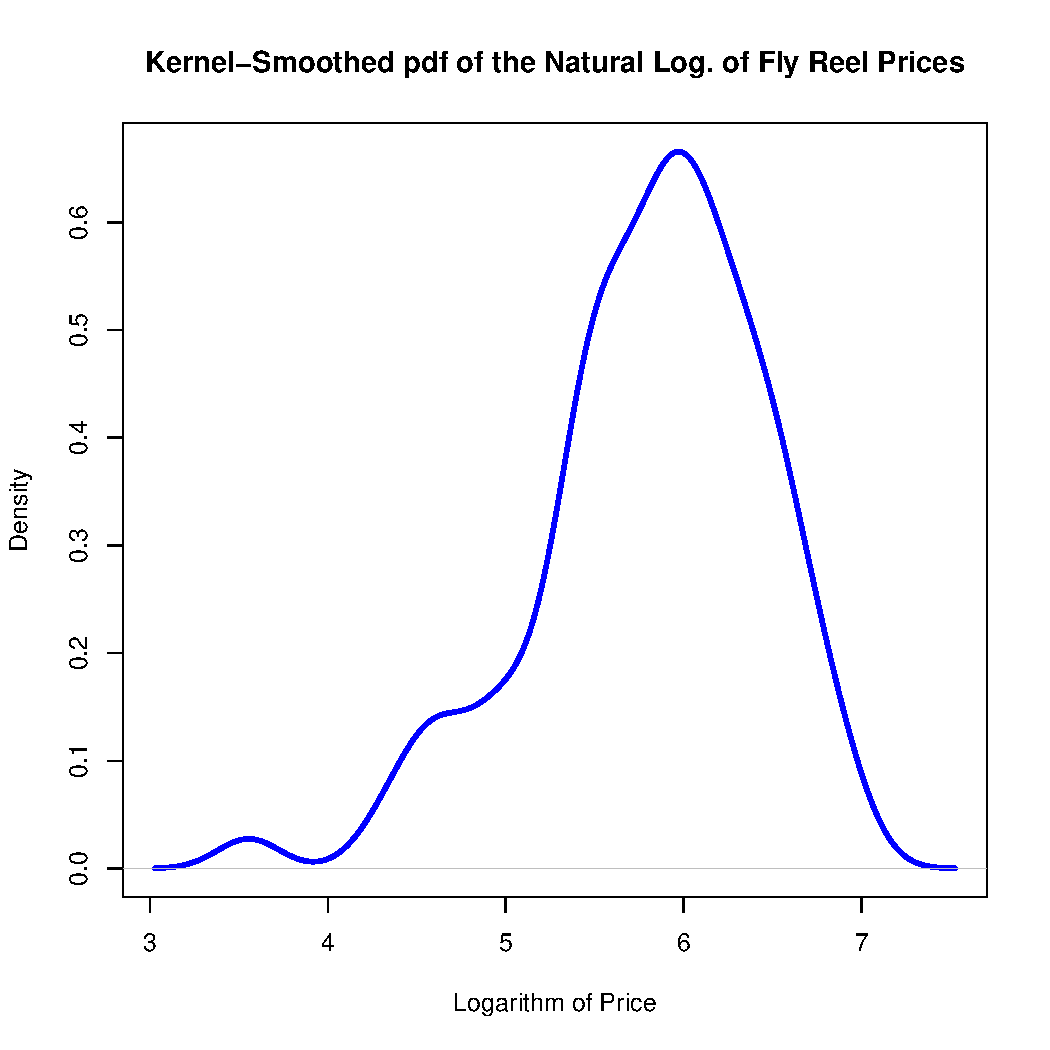
\includegraphics[scale = 0.5, keepaspectratio=true]{../Figures/density_log_prices}
  \caption{Probability Density Function of the Logarithm of Fly Reel Prices} \label{fig:density_log_prices}
\end{figure}




\pagebreak
\section*{Normality of the Original and Transformed Variables}

Figure \ref{fig:qq_prices} shows a pair of Q-Q plots, 
comparing quantiles of the empirical distribution against
the quantiles of the normal distribution. 
In the left panel, Figure \ref{subfig:qq_prices} shows this comparison 
for the original level of the fly reel prices, without transformation. 
In the right panel, Figure \ref{subfig:qq_log_prices} shows this comparison 
for the logarithmic transformation of fly reel prices, without transformation. 
Consistent with the pair of distributions estimated above, 
each plot shows a divergence from a normal distribution,
suggesting that an optimal transformation might lie somewhere in the middle.
The Box-Cox transformation allows for this possibility. 

\begin{figure}[!ht]
\subfloat[Fly Reel Prices\label{subfig:qq_prices}]{%
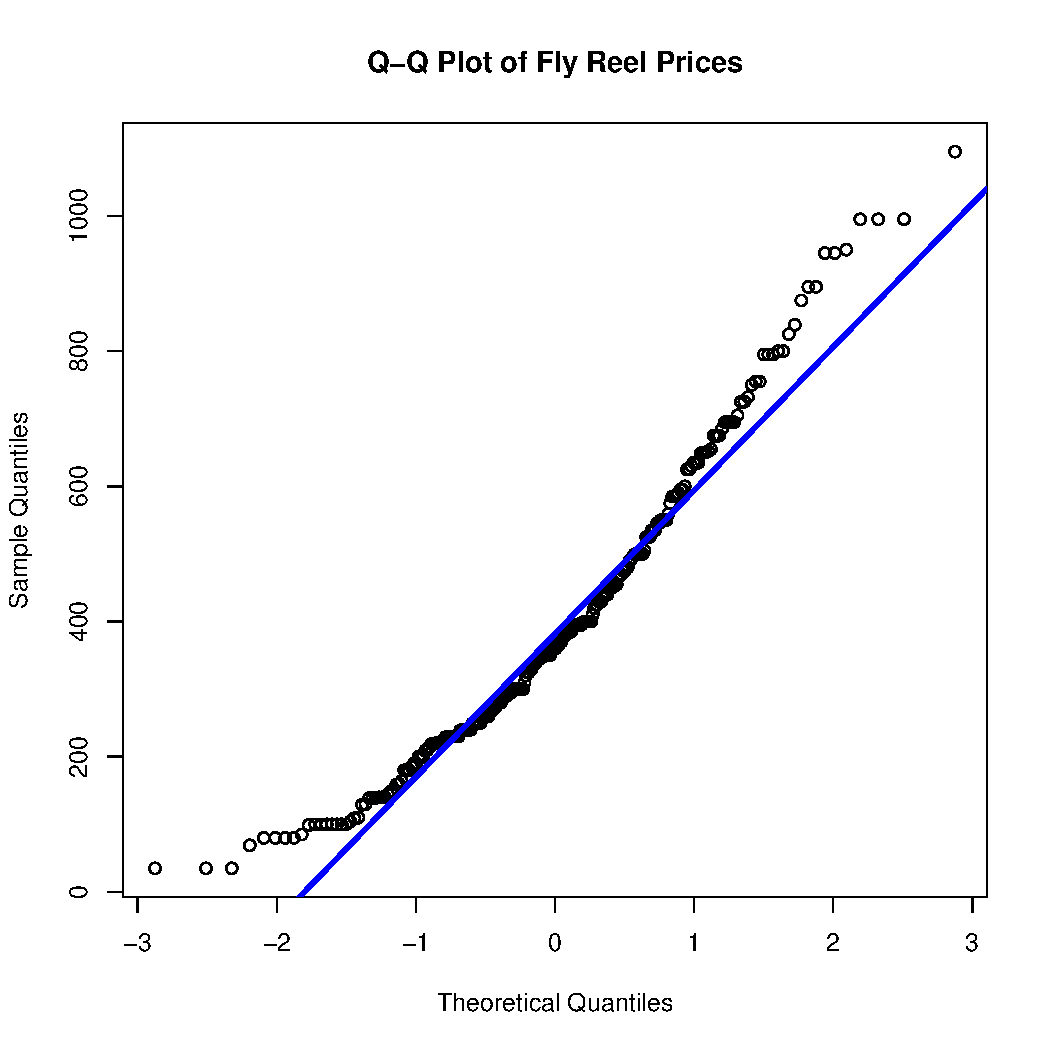
\includegraphics[width=0.5\textwidth]{../Figures/qq_prices}}
\hfill
\subfloat[Transformed Fly Reel Prices\label{subfig:qq_log_prices}]{%
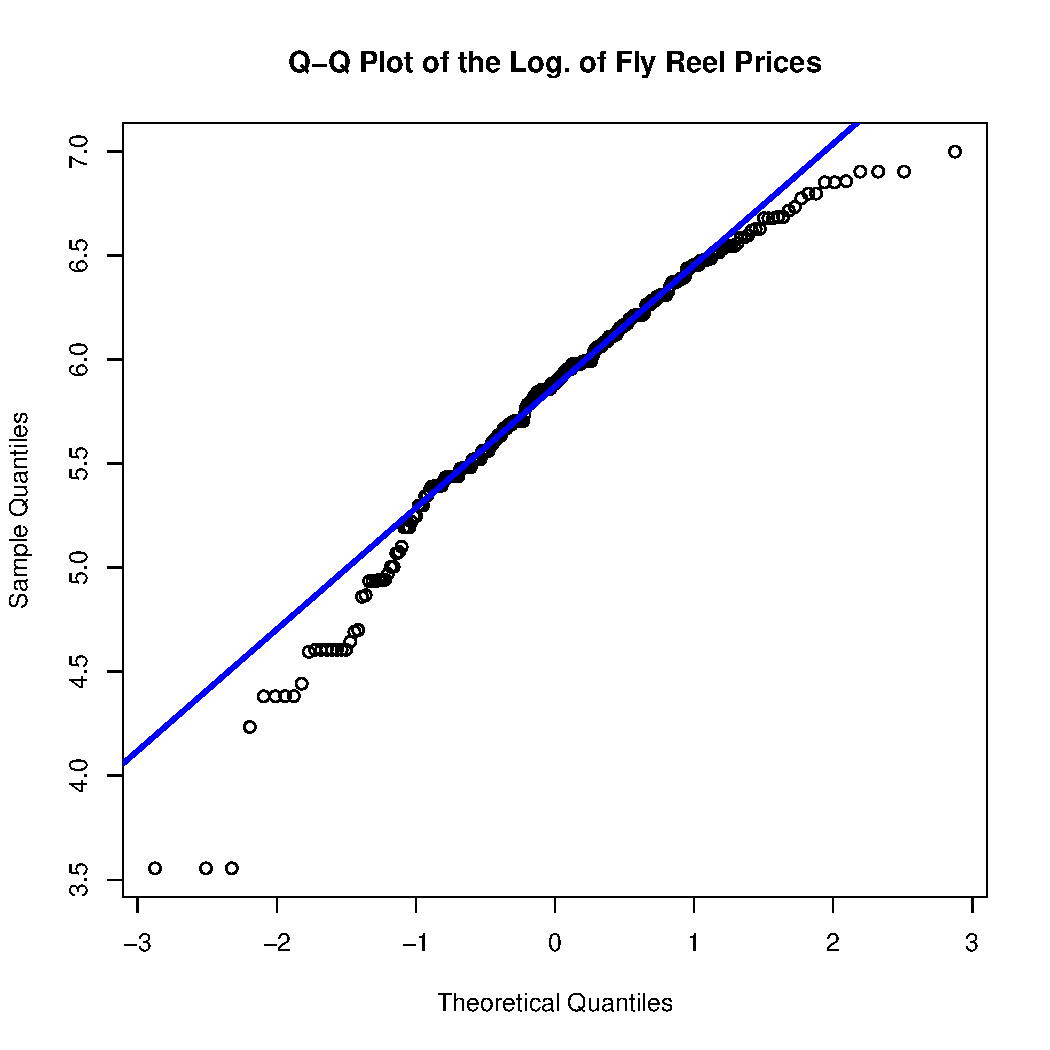
\includegraphics[width=0.5\textwidth]{../Figures/qq_log_prices}}

\caption{Q-QPlots of the Log. and Levels of Fly Reel Prices}
\label{fig:qq_prices}
\end{figure}



%%%%%%%%%%%%%%%%%%%%%%%%%%%%%%%%%%%%%%%%
% Box-Cox Transformation
%%%%%%%%%%%%%%%%%%%%%%%%%%%%%%%%%%%%%%%%


\pagebreak
\section{Box-Cox Transformation of Fly Reel Prices}

Under the Box--Cox transformation of $P_n$, the price of reel $n$
is calculated as follows,
$$\Lambda(P_n)\equiv
  \begin{cases}
	\frac{P_n^\lambda-1}{\lambda}	& \textrm{if } \lambda > 0 \\
           \log P_n                     			& \textrm{if } \lambda = 0.\\
  \end{cases}
$$
The following code block defines a function that performs a
Box-Cox transformation.

\vspace{1.0in}

\begin{lstlisting}[language=R]
# Box-Cox transformation.
Lambda_Price <- function(price, lambda) {
  if (lambda == 0) {
    return(log(price))
  } else {
    return((price^lambda - 1)/lambda)
  }
}
\end{lstlisting}

\pagebreak
\subsection{Log-likelihood Function}

Under the Box-Cox transformation,
the fly reel prices can be decomposed into a location parameter $\mu^0$ 
and an error $U$, so
$$\Lambda(P_n) = \mu^0(\lambda) + U_n,$$
where the $U_n$s are independent, mean-zero, constant-variance 
$\sigma^2(\lambda)$, Gaussian (normal) errors. 
In the above equation, for clarity, the dependence of $\mu^0$ and 
$\sigma^2(\lambda)$ on $\lambda$ is made explicit.


The next code block defines a likelihood function for the normal distribution of the errors
as a function of the parameter $\lambda$.

\begin{lstlisting}[language=R]
log_like_uni <- function(price, lambda) {

  # Calculate maximum likelighood estimates of the parameters.
  n <- length(price)
  lambda_price <- Lambda_Price(price, lambda)
  mu_0_lambda <- mean(lambda_price)
  sigma_2_lambda <- sum((lambda_price - mu_0_lambda)^2)/n

  # Calculate the log-likelihood from the sum of the logarithms
  # of the density of the normal distribution.
  like <- - n/2*log(2*pi*sigma_2_lambda)
  like <- like - 1/2/sigma_2_lambda*sum((lambda_price - mu_0_lambda)^2)
  like <- like + (lambda - 1)*sum(log(price))
  return(like)
}
\end{lstlisting}

\pagebreak
As a first approximation, 
One can calculate the value of the log-likelihood function on a grid of values
to find an optimal value of $\lambda$.
The plot of this likelihood function is shown in Figure \ref{fig:box_cox_loglike_uni}.
The red points represent the values of the log-likelihood 
at the optimum $\lambda = 0.43$ and at $\lambda = 0$ and $\lambda = 1$.

\begin{lstlisting}[language=R]
# Calculate values of the log-likelihood function.
lambda_grid <- seq(-1, 2.5, by = 0.001)
like_grid <- 0*lambda_grid
for (lambda_num in 1:length(lambda_grid)) {
  like_grid[lambda_num] <- log_like_uni(price = flyreels[, 'Price'],
                                    lambda = lambda_grid[lambda_num])
}
\end{lstlisting}

\begin{figure}[h!]
  \centering
  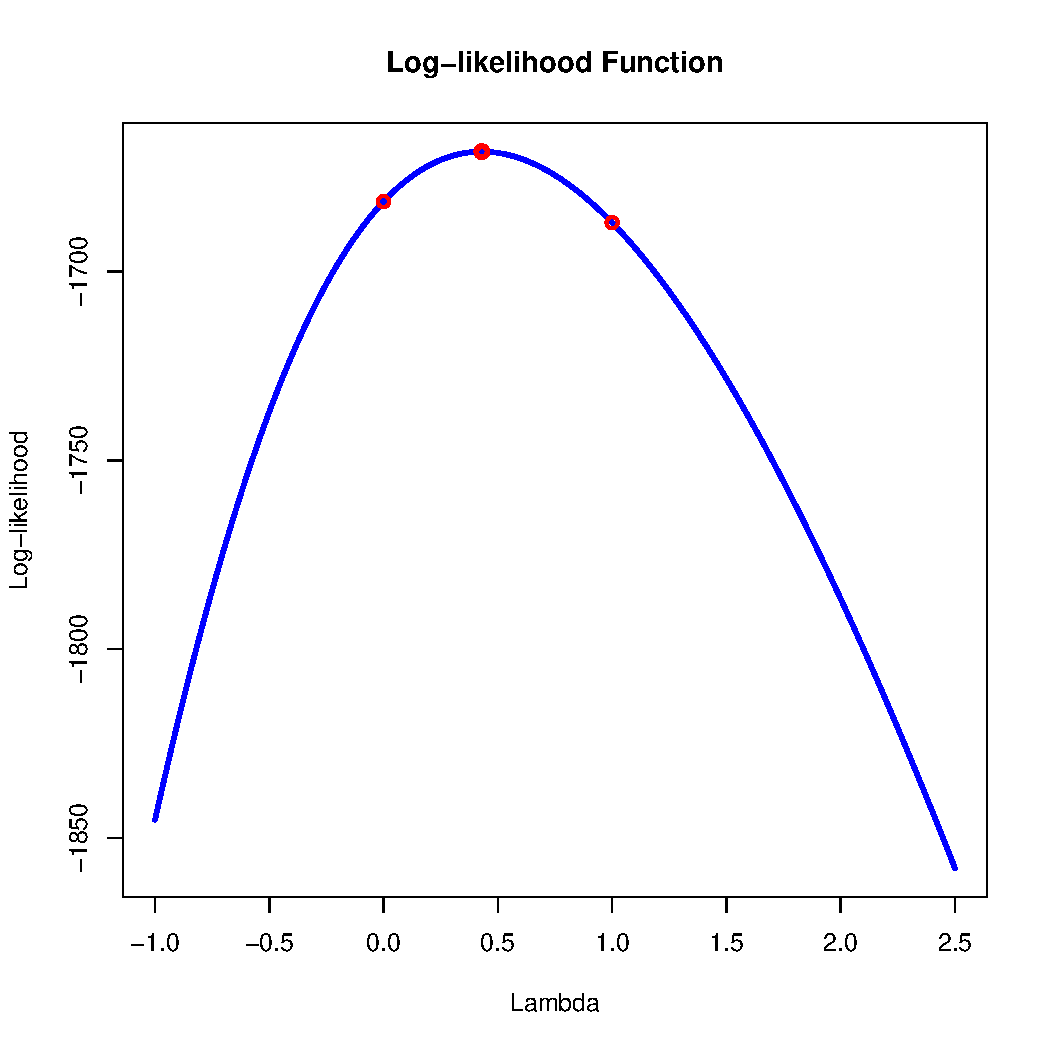
\includegraphics[scale = 0.5, keepaspectratio=true]{../Figures/box_cox_loglike_uni}
  \caption{Log-likelihood Function for Box-Cox Transformation} \label{fig:box_cox_loglike_uni}
\end{figure}


\pagebreak
\subsection{Testing for an Appropriate Transformation}

Now we consider the statistical properties of these estimates
by calculating a likelihood ratio statistic.

\begin{lstlisting}[language=R]
> # Calculate likelihood ratio statistics.
> LR_stat_0 <- - 2*(like_mu_0 - like_MLE)
> print(LR_stat_0)
[1] 26.4604
> LR_stat_1 <- - 2*(like_mu_1 - like_MLE)
> print(LR_stat_1)
[1] 37.62182
> 
> 
> # Compare to quantile of chi-squared distribution with 1 degree of freedom.
> LR_cv_5 <- qchisq(p = 0.95, df = 1)
> print(LR_cv_5)
[1] 3.841459
> 
> # Calculate p-values for these tests.
> p_value_0 <- 1 - pchisq(q = LR_stat_0, df = 1)
> print(p_value_0)
[1] 2.689959e-07
> p_value_1 <- 1 - pchisq(q = LR_stat_1, df = 1)
> print(p_value_1)
[1] 8.58782e-10
> 
\end{lstlisting}

Statistically, this is evidence to reject them both.
This suggests using the transformation at the MLE.
However, one may want to investigate further 
to find out whether it is worth 
transforming the data. 
There exists a trade-of between interpretability and 
the accuracy of the statistical specification. 


\clearpage
\section{\textsf{R} Packages for the Box-Cox Transformation}
\subsection*{Using the \texttt{MASS} Package}

As an illustration, we calculated
the likelihood ourselves.
However, there exist other packages
to output the estimation results for
an optimal Box-Cox transformation.

One option is to use the function from the \texttt{MASS} package.
This is an \textsf{R} package that accompanies a well-know statistics textbook
and has a great reputation. 
In the \texttt{MASS} package, the notation is the same as for a linear model.


\begin{lstlisting}[language=R]
# In the MASS package, the notation is the same as for a linear model.
# i.e., summary(lm(Price ~ 1, data = flyreels))
bc_grid_MASS <- MASS::boxcox(Price ~ 1,
                             data = flyreels,
                             lambda = lambda_grid)
\end{lstlisting}

The output is plotted in Figure \ref{fig:plot_like_MASS}.

\begin{figure}[h!]
  \centering
  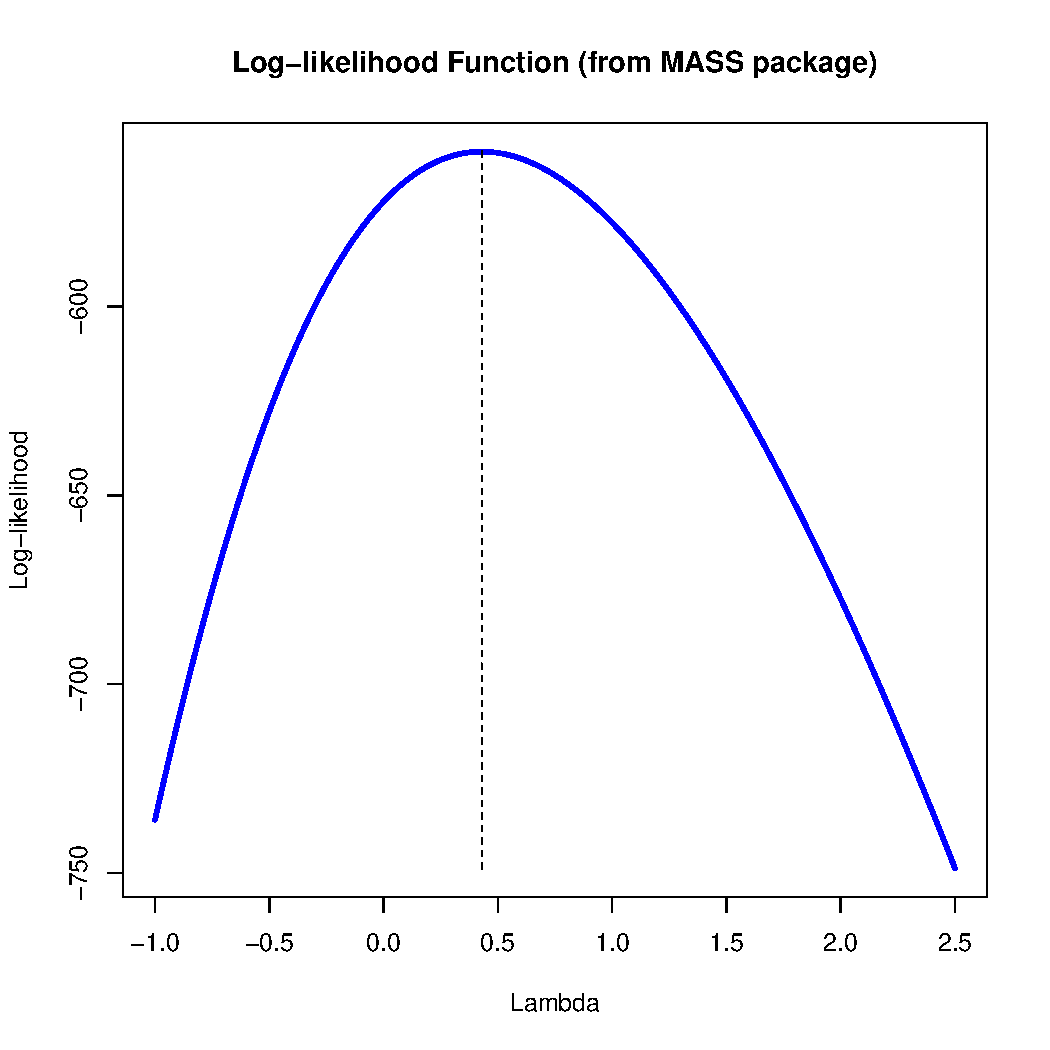
\includegraphics[scale = 0.5, keepaspectratio=true]{../Figures/plot_like_MASS}
  \caption{Log-likelihood Function for Box-Cox Transformation (\texttt{MASS} package)} \label{fig:plot_like_MASS}
\end{figure}


\clearpage
\section*{Using the \texttt{car} Package}

The \texttt{car} package is another well-known option.
With this function, the optimization produces 
a figure automatically from the code below.

\begin{lstlisting}[language=R]
bc_grid_car <- car::boxCox(object = lm(data = flyreels,
                                       formula = Price ~ 1),
                           lambda = lambda_grid)
\end{lstlisting}

The output is plotted in Figure \ref{fig:plot_like_car}.

\begin{figure}[h!]
  \centering
  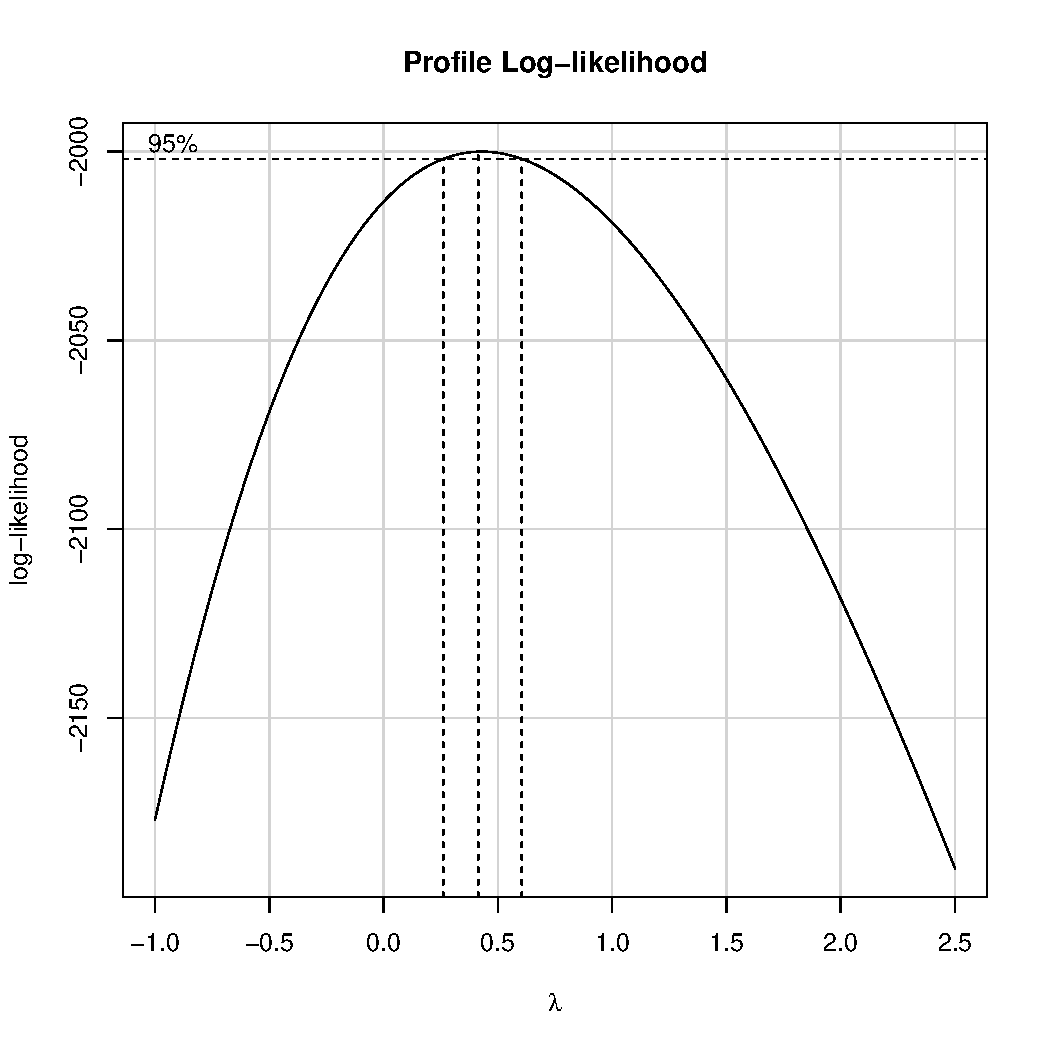
\includegraphics[scale = 0.5, keepaspectratio=true]{../Figures/plot_like_car}
  \caption{Log-likelihood Function for Box-Cox Transformation (\texttt{car} package)} \label{fig:plot_like_car}
\end{figure}


\clearpage
\section*{Using the \texttt{EnvStats} Package}


The \texttt{EnvStats} package is another option
but it is one designed for environmental statistics.
That is, it is not a generic package designed for the population of statisticians at large.
For that reason, it is missing some of the features that
a statistician would expect.
The notation and interpretation, however, are similar, 
except that the straight call to \texttt{boxcox}
simply does the calculation, 
unless you specify otherwise.

\begin{lstlisting}[language=R]
> # Find optimal value of lambda.
> bc_grid_ES_opt <- EnvStats::boxcox(x = flyreels[, 'Price'],
+                                    lambda = range(lambda_grid),
+                                    optimize = TRUE,
+                                    objective.name = "Log-Likelihood")
> 
> bc_grid_ES_opt$lambda
[1] 0.4295551
> 
\end{lstlisting}


The output is plotted in Figure \ref{fig:plot_like_EnvStats}.

\begin{figure}[h!]
  \centering
  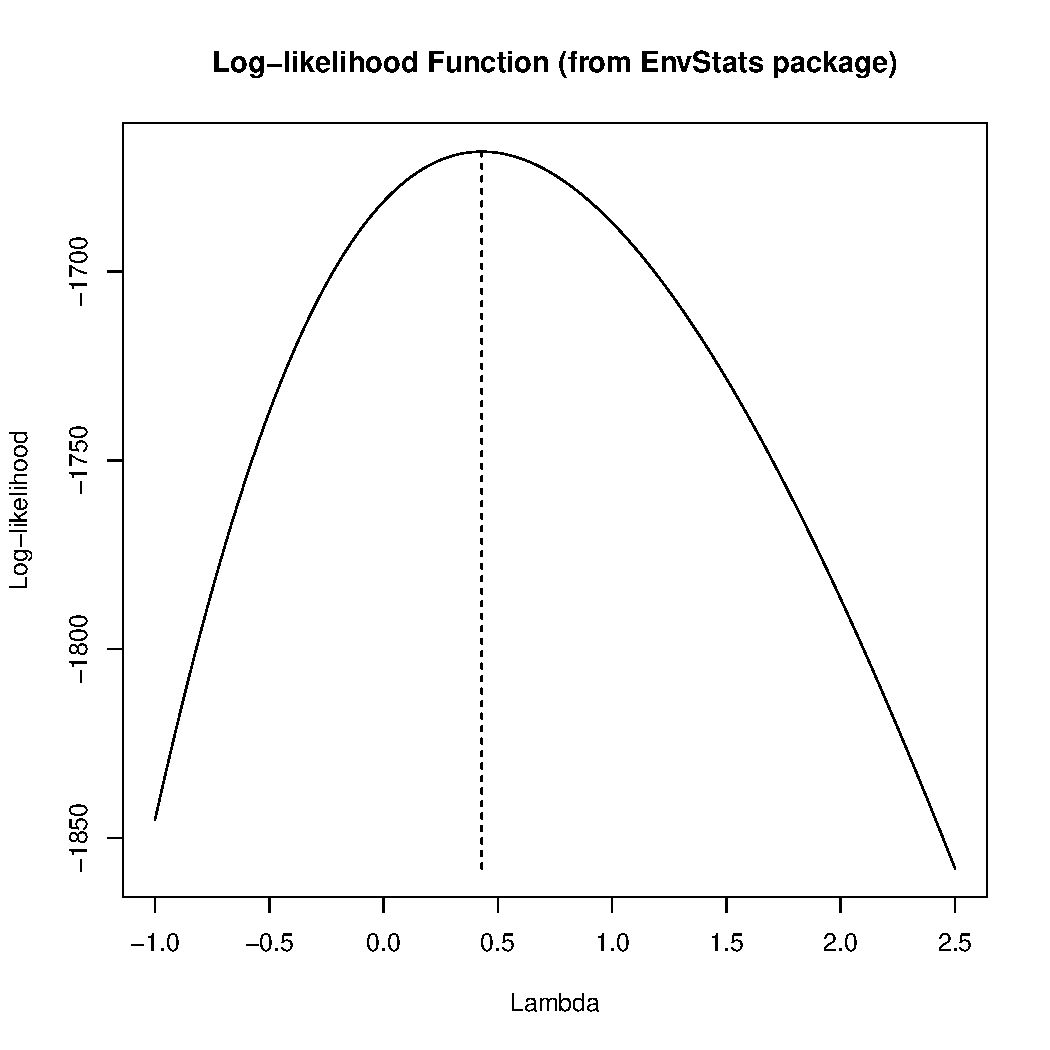
\includegraphics[scale = 0.5, keepaspectratio=true]{../Figures/plot_like_EnvStats}
  \caption{Log-likelihood Function for Box-Cox Transformation (\texttt{EnvStats} package)} \label{fig:plot_like_EnvStats}
\end{figure}






\clearpage
\section*{Normality of the Transformed Variable}

Now compare the quantiles of the distribution of the transformed variable with 
the original. 
We already plotted normal QQ plot for fly reel prices when considering the log transformation.
Now we can generate a new dependent variable with the results from the estimates above.


\begin{lstlisting}[language=R]
# Generate new dependent variable with results from estimates above.
flyreels[, 'Trans_Price'] <- Lambda_Price(price = flyreels[, 'Price'],
                                          lambda = lambda_hat)
\end{lstlisting}

Figure \ref{fig:qq_prices} shows this comparison
and the panel on the right, Figure \ref{subfig:qq_boxcox}, 
shows that the quantiles of the distribution of the transformed variable
nearly overlap with those of the normal distribution.
From a purely statistical perspective, 
this provides evidence that the prices are best modeled with the transformation
at the optimal $\lambda = 0.43$.
From a practical point of view, however, 
it is still an open question whether this 
added complexity is warranted when other variables are added to the model. 


\begin{figure}[!ht]
\subfloat[Fly Reel Prices\label{subfig:qq_prices}]{%
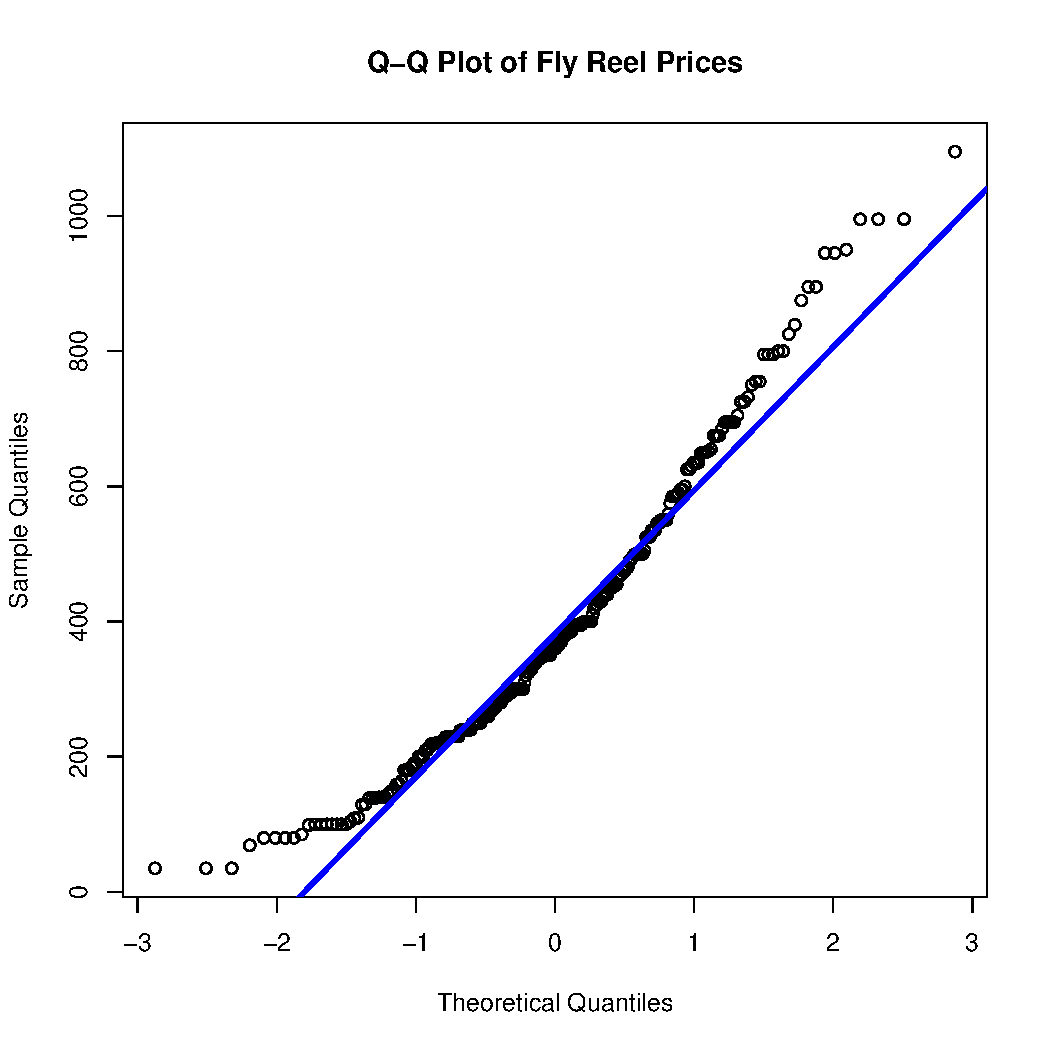
\includegraphics[width=0.5\textwidth]{../Figures/qq_prices}}
\hfill
\subfloat[Transformed Fly Reel Prices\label{subfig:qq_boxcox}]{%
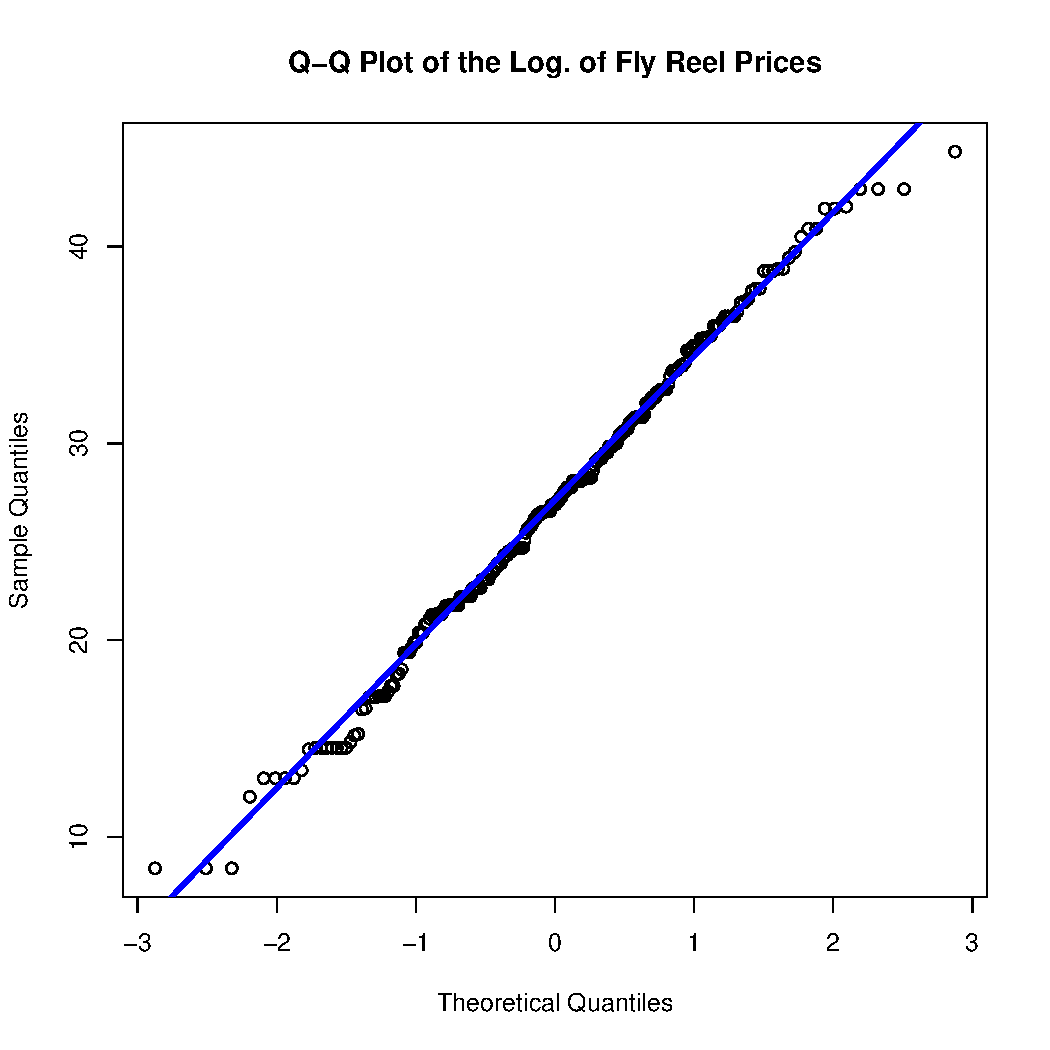
\includegraphics[width=0.5\textwidth]{../Figures/qq_boxcox}}

\caption{Q-QPlots of the Transformed Fly Reel Prices}
\label{fig:qq_prices}
\end{figure}








%%%%%%%%%%%%%%%%%%%%%%%%%%%%%%%%%%%%%%%%
\end{document}
%%%%%%%%%%%%%%%%%%%%%%%%%%%%%%%%%%%%%%%%
